\documentclass{article}

\usepackage[preprint]{tmlr}
% \usepackage{tmlr}
% \usepackage[accepted]{tmlr}
\usepackage{amsmath,amssymb,amsfonts}
\usepackage{booktabs,array,tabularx,multirow}
\usepackage{graphicx,microtype,xcolor}
\usepackage{hyperref,url}
\hypersetup{hidelinks}
\graphicspath{{figs/}}

\newcommand{\records}{\ensuremath{\mathsf{Records}}}
\newcommand{\values}{\ensuremath{\mathsf{Values}}}
\newcommand{\groups}{\ensuremath{\mathsf{Groups}}}
\newcommand{\numbertype}{\ensuremath{\mathsf{Number}}}
\newcommand{\valuetype}{\ensuremath{\mathsf{Value}}}
\newcommand{\booltype}{\ensuremath{\mathsf{Bool}}}
\newcommand{\ranking}{\ensuremath{\mathsf{Ranking}}}

\title{Building an Executable and Auditable Reasoning Environment for Verification-Guided Improvement}
\author{\name Hai Zhou \email uceeh01@ucl.ac.uk \\
 \addr University College London}
\def\month{08}
\def\year{2026}
\def\openreview{}

\begin{document}
\maketitle

\begin{abstract}
An answer that changes after feedback does not by itself show that an agent found and corrected an
error.  The change may come from resampling, different retrieval, additional computation, or access
to protected information.  Studying verification guided improvement therefore requires an
environment in which the proposed reasoning action, its consequence, and the authority of the
feedback are observable.  We build such an environment for UK public procurement.  Its state is a
versioned, provenance preserving graph, its actions are typed programs, its transitions are
deterministic executions, and its feedback separates runtime checks from offline oracle agreement
and constraint audits.  The environment contains 215,221 contract award records and supports a
12,828 question program first benchmark with explicit non answer states.  It is distinct from the
repair and learning mechanisms evaluated on top of it.

Across four protocols, the environment reveals both useful gains and their limits.  On the primary
2,025 question non development evaluation, the strongest fully local system reaches 85.73\%,
compared with 69.19\% for its cloud teacher and 38.42\% for top 40 retrieval.  A fixed plan replay
shows that one deterministic grounding intervention raises correct executions from 89 to 103 of
136 without degrading an initially correct plan.  Supervised fine tuning improves both Qwen and
Llama planners, while later continuation and preference stages are not monotonic.  Yet 1,262
answer producing traces that pass the online runtime fail an offline oracle or answer shape check,
and 56 of 229 mechanically audited repair targets omit a mapped question constraint.  Separate
PACS and WikiTableQuestions protocols test compositional robustness and cross domain portability.
The environment does not create or certify improvement.  It makes reasoning actions, execution
traces, and feedback pathways observable enough to locate gains and verification boundaries.
\end{abstract}

\section{Introduction}
\label{sec:introduction}

When an agent answers correctly after receiving feedback, the outcome permits several
explanations.  The feedback may have identified the error, but the agent may also have sampled a
lucky answer, changed the evidence it saw, spent more computation, or used information that should
have remained hidden.  Final accuracy records the outcome and not the path that produced it.  This
is a measurement problem before it is a modelling problem.  A controlled study of improvement
needs a stable state, an explicit action, a replayable transition, and feedback whose authority is
known.  Recent benchmarks make this separation central when studying data centric post training,
persistent personal agents, and agents that modify other agents
\citep{meng2026rsibench,xue2026past,mishra2026aie}.  We study a narrower question.  Can an
executable data environment make verification guided changes in reasoning observable and
attributable without treating successful execution as proof of meaning?

Public procurement turns the measurement problem into a concrete reasoning problem.  Questions
about who bought what from whom often require role sensitive joins, complete populations, set
operations, ranking, and exact aggregation.  A retriever can return relevant records without
returning the complete set over which a count or sum is defined.  A program generator fails in a
different way.  It can emit a valid program that executes successfully after reversing buyer and
supplier roles or stopping one relation too early.  Figure~\ref{fig:motivation} shows both failures
on one saved procurement question.  Top 40 retrieval includes the 23 records naming the supplier
but its reader answers 14.  A valid one hop program answers 23.  The intended bridge first derives
16 buyers and then enumerates 4,257 notices.  The contrast is not simply text versus structured
data.  It is the difference between observing a plausible output and observing the action and the
population that produced it.

\begin{figure}[t]
  \centering
  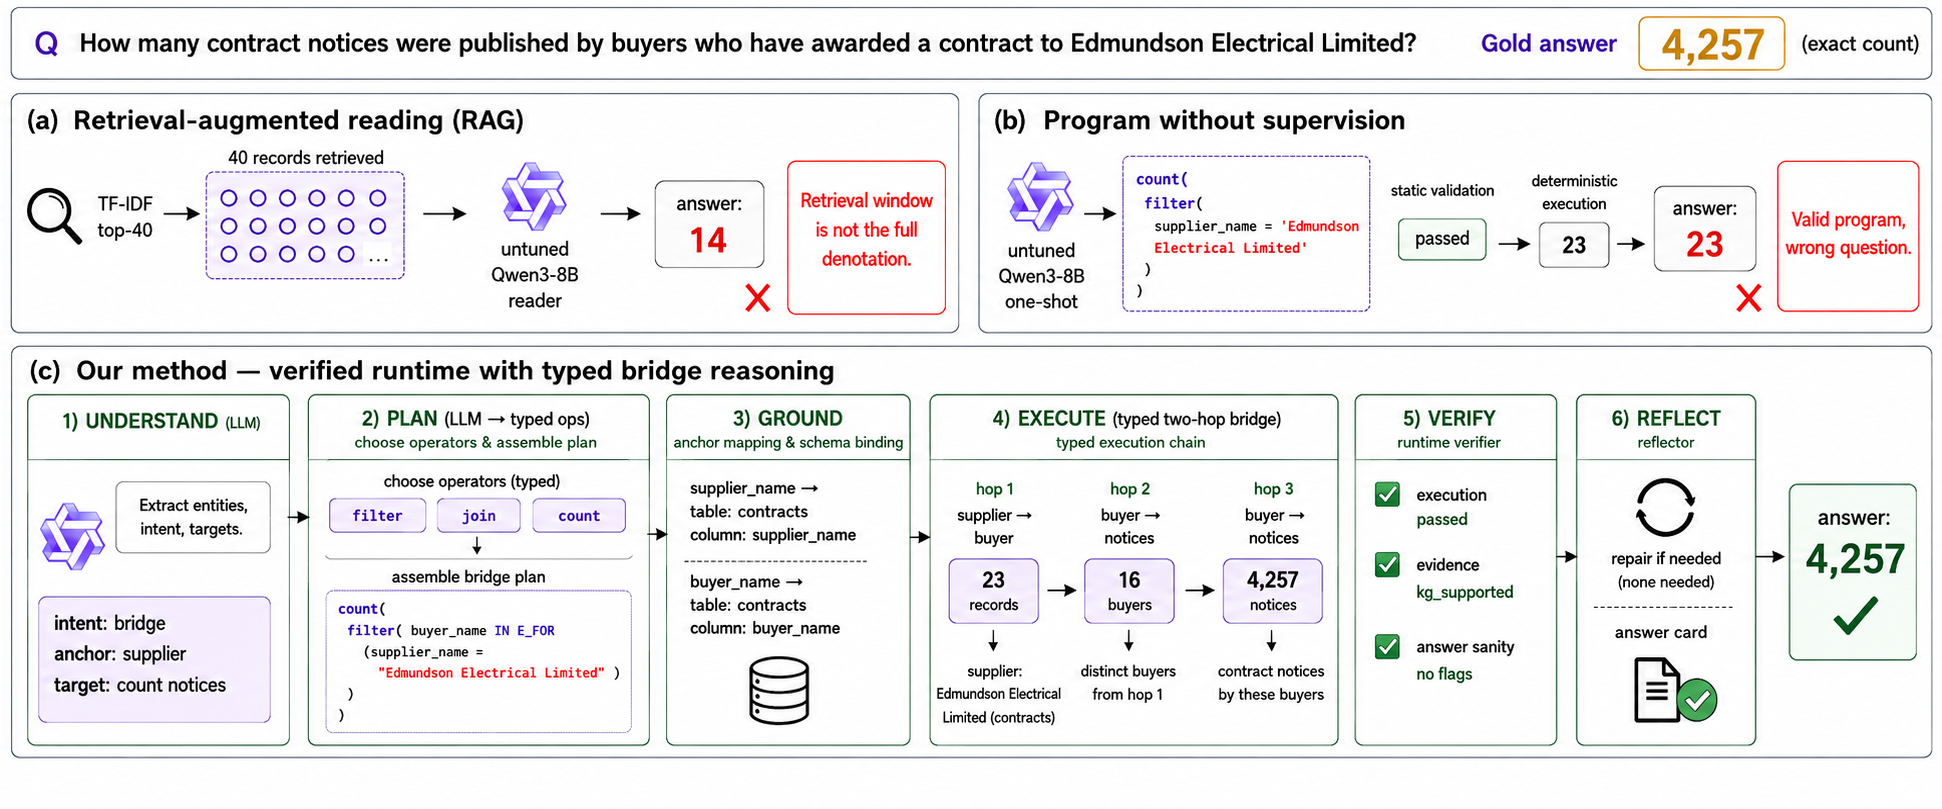
\includegraphics[width=0.96\linewidth]{fig01_environment.png}
  \caption{A single question exposes the two ambiguities that motivate the environment.  Finite
  retrieval does not recover the complete target population, while an executable one hop program
  answers a different question.  The complete bridge records the intermediate populations before
  returning 4,257.  The displayed gold answer is used only by offline evaluation.  The online panel
  reports execution, evidence, and output consistency checks rather than semantic certification.}
  \label{fig:motivation}
\end{figure}

We build an executable reasoning environment in which these distinctions are first class objects.
The state is a frozen graph derived from UK Open Contracting Data Standard releases.  An action is a
typed intent or graph program.  The transition is deterministic execution over the full selected
population.  The observation contains grounded constraints, intermediate set sizes, the denotation,
and provenance identifiers.  Feedback is layered.  Syntax, schema, grounding, execution, and
release information are available online without an answer oracle.  Expected answer shape and
typed oracle agreement are used only during offline curation, while explicit constraint retention
is audited separately.  Repair, supervised fine tuning, rejection sampling, and preference
optimisation operate on top of this environment.  They are not part of its definition.

This separation leads to a two sided empirical result.  The full local runtime is substantially
more accurate than the stored retrieval and cloud systems on 2,025 questions not used for model
selection.  A narrow fixed plan intervention directly repairs one class of unsafe sums, and
supervised fine tuning improves both tested model families.  At the same time, online acceptance
admits 1,262 candidates later rejected by offline checks, an audit finds omitted constraints in 56
of 229 mapped repair targets, and later learning stages do not improve monotonically.  We call this
separation between successful execution and preservation of the requested computation the
\emph{execution faithfulness gap}.  PACS then tests new compositions and alternative surfaces under
a separate single call protocol, while WikiTableQuestions tests whether the recursive algebra can
move beyond procurement.

The paper makes three contributions.  First, it constructs a versioned structured reasoning
environment over procurement data in which typed actions execute deterministically and can be
replayed through intermediate populations and source provenance.  Second, it introduces a layered
measurement contract that keeps online runtime authority, offline oracle agreement, and constraint
faithfulness separate, together with a program first benchmark that scores answerable and non
answerable cases.  Third, it evaluates complete systems, fixed plan repair, checked trace learning,
compositional robustness, and cross domain transfer under distinct protocols.  The purpose of this
separation is not to attach every gain to verification.  It is to state which gain each experiment
can support and where that evidence ends.

\section{Related Work}
\label{sec:related}

\paragraph{Environments for studying improvement.}
Recent work has shifted from asking only whether an agent solves a task to asking whether a
controlled process makes the agent or its apparatus better.  RSIBench Data fixes training,
serving, evaluation, and budgets so that changes can be attributed to data research decisions
\citep{meng2026rsibench}.  PAST Bench uses matched persistence conditions and trace evidence to
separate later task gains from the mechanism intended to produce them \citep{xue2026past}.
AIE Bench fixes the evaluation framework while a meta agent modifies a target agent
\citep{mishra2026aie}.  TangramSR supplies a continuous geometric state and an oracle guided
refinement loop \citep{tan2026tangramsr}.  These studies establish an important design principle.
Improvement becomes interpretable only when the mutable object and the surrounding evaluation
conditions are separated.  Their environments mainly concern code, persistence, agent scaffolds,
or synthetic geometry.  Real world compositional data reasoning adds a different requirement.
The state itself must define identity, roles, completeness, aggregation, and provenance before an
action has a stable meaning.

\paragraph{Executable reasoning over structured data.}
Semantic parsers map questions to logical forms over tables, databases, and knowledge graphs
\citep{pasupat2015compositional,wang2020ratsql,cheng2023binder}.  Other systems combine language
models with schemas, relation paths, or structured data tools
\citep{jiang2023structgpt,luo2024chatkbqa,luo2024rog}.  Constrained decoding prevents illegal
prefixes \citep{scholak2021picard,dong2024xgrammar}, while executors move factual calculation out
of free form generation.  These techniques make a proposal inspectable, but they do not by
themselves define what an entity, field, amount, or relation means.  In procurement, the same body
may appear under many platform identifiers and several monetary fields may repeat the same value.
An executable program is meaningful only relative to explicit data conventions.

\paragraph{Execution feedback and learning.}
Execution has been used to rank programs, train correctors, and filter generated supervision
\citep{ni2023lever,wang2021executions,zhu2026scd}.  STaR, ReST, execution filtered SQL training,
and preference learning similarly retain candidates that satisfy an acceptance rule
\citep{zelikman2022star,gulcehre2023rest,zhang2025exesql,zhai2025excot}.  Denotation supervision is
nevertheless incomplete because different programs can produce the same answer
\citep{pasupat2016denotations,lee2023spurious}.  Our concern is therefore not whether execution is a
useful signal.  It is how much authority that signal should have when the same environment supports
answer release, repair, and training data selection.

\paragraph{Procurement, provenance, and answerability.}
TheyBuyForYou demonstrates how procurement and company records can be integrated as linked data
for search and analysis \citep{soylu2022theybuyforyou}.  We use procurement as a realistic
reasoning substrate rather than as an example database.  It stresses complete population access,
role dependent joins, entity ambiguity, and value provenance at the same time.  Explicit ambiguous,
unsupported, and empty result cases connect the benchmark to unanswerable and selective question
answering \citep{rajpurkar2018know,kamath2020selective}.  The remaining gap is an environment that
exposes a typed reasoning action, executes it against a convention explicit snapshot, returns
traceable observations, and keeps runtime feedback distinct from correctness and faithfulness.

\section{The Executable Reasoning Environment}
\label{sec:contract}

\subsection{Environment contract}

We define the environment as
\begin{equation}
  \mathcal{E}=(K,\mathcal{Z},T,O,F).
  \label{eq:environment}
\end{equation}
The state $K$ is a frozen, versioned procurement graph.  The action space $\mathcal{Z}$ contains
typed programs and explicit non answer actions.  The transition $T(K,z)$ grounds and executes an
action $z$ without changing $K$.  The observation $O(K,z)$ contains the execution status,
intermediate populations, denotation, and provenance references.  Feedback $F$ is not a scalar
reward.  It is a collection of judgements with different information and authority.

For a fixed state and grounded program, the transition is replayable.
\begin{equation}
  T_v(K,z)=T_v(K,z)^{\prime}
  \quad\text{when the snapshot, program, and executor version $v$ are unchanged.}
  \label{eq:replay}
\end{equation}
This statement does not make language model planning deterministic.  It says that once an action
has been proposed, its data consequence is fixed and can be attributed to that action.

\subsection{Feedback authority}

The online contract records four ordered judgements
\begin{equation}
  f_{\mathrm{valid}},\quad f_{\mathrm{ground}},\quad
  f_{\mathrm{execute}},\quad f_{\mathrm{release}}.
  \label{eq:online}
\end{equation}
Validity covers program structure, types, references, and dependency order.  Grounding maps fields,
values, roles, entities, and guards to the backend contract.  Execution reports whether the
grounded action reaches a denotation.  Release records output consistency, evidence availability,
and disclosure conditions.  No online judgement reads the benchmark answer.  A repairable
structural failure may condition one revised proposal, after which the entire deterministic path is
run again.  A clean empty result, ambiguity, or unsupported request terminates rather than inviting
answer search.

Offline analysis adds oracle agreement $f_{\mathrm{oracle}}$ and expected answer shape
$f_{\mathrm{shape}}$.  The oracle may filter or label a trace, but its value is removed before any
student target is exported.  Constraint faithfulness $f_{\mathrm{constraint}}$ remains a separate
audit because neither execution nor denotation agreement proves that every explicit condition in
the question survives in the program.  The resulting distinction is
\begin{equation}
  (f_{\mathrm{valid}}\wedge f_{\mathrm{ground}}\wedge f_{\mathrm{execute}})
  \not\Rightarrow f_{\mathrm{oracle}},
  \qquad
  f_{\mathrm{oracle}}\not\Rightarrow f_{\mathrm{constraint}}.
  \label{eq:authority}
\end{equation}
Figure~\ref{fig:online-offline} shows where these judgements enter the system.

\begin{figure}[t]
  \centering
  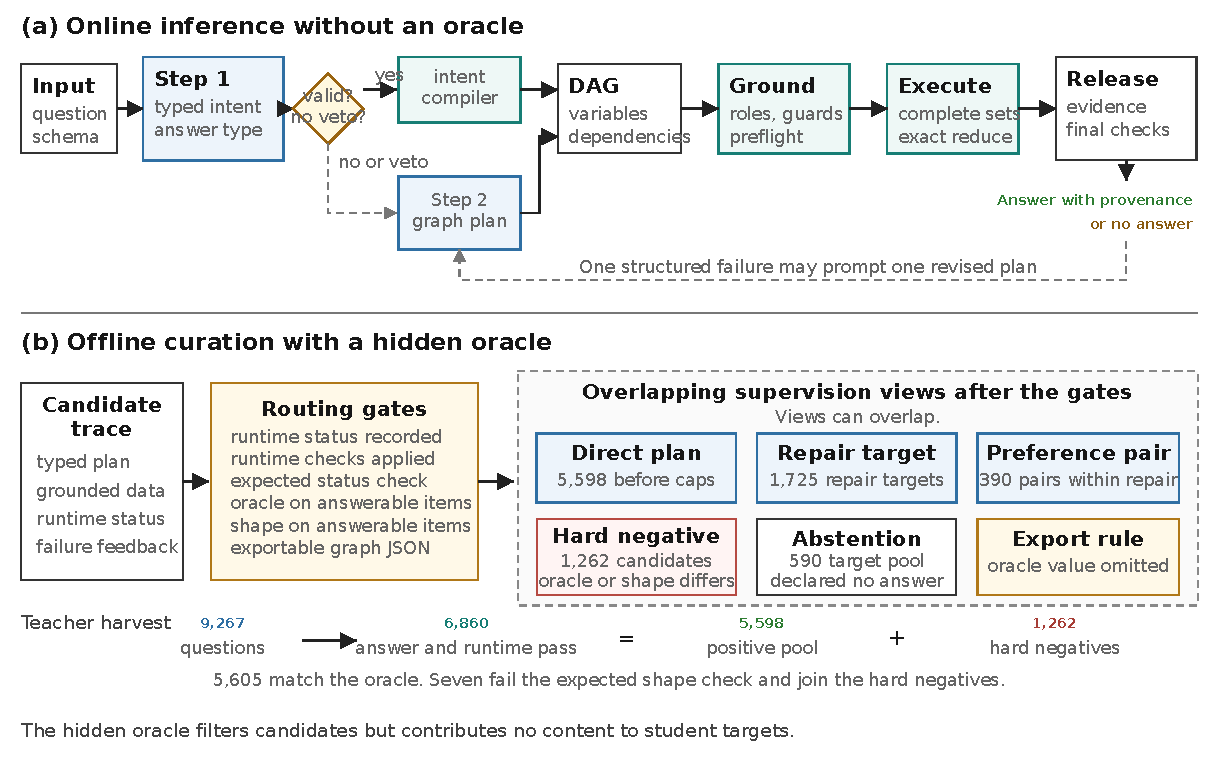
\includegraphics[width=0.86\linewidth]{fig02_online_offline}
  \caption{The online and offline pathways have different authority.  Online inference proposes,
  grounds, executes, and releases without an answer oracle.  Offline curation additionally checks
  expected status, answer shape, and hidden oracle agreement before routing overlapping supervision
  views.  Oracle values do not enter student targets.}
  \label{fig:online-offline}
\end{figure}

\subsection{Task and answer contract}

For question $q$ over snapshot $K$, the system predicts a typed denotation $\hat y$ or a declared
non answer state.  Boolean answers remain Boolean, numeric answers use decimal equality, sets
compare normalised members, and rankings preserve order.  The benchmark distinguishes three non
answer cases.  An unsupported question requests an operation outside the contract.  An ambiguous
question admits more than one defensible interpretation.  A no result question is well formed but
has an empty denotation in $K$.  These labels describe the declared snapshot and do not claim that
the public record outside it has no answer.

\section{Building the Environment}
\label{sec:building}

\subsection{A versioned procurement state}

The source collection contains 166,277 compiled OCDS releases in five annual files spanning 2022
to 2026 \citep{ocds}.  The loader streams each file, discards rows without a usable process
identifier or date, and retains the latest dated release for each OCID.  A second extraction pass
accepts only the selected OCID and release identifier pair.  This creates a current snapshot and
does not preserve amendment history.

Organisation resolution proceeds in ordered, precision oriented tiers.  Recognised official
scheme identifiers anchor canonical rows.  A platform identifier can attach to an official entity
only when observations with the same process, normalised name, and party role point to one
candidate.  Curated exact lookup, exact name and region, and exact name without region handle the
remaining observations.  Residuals stay as provisional singletons.  A later offline extension
applies reviewed deterministic and model adjudicated candidate merges only when component level
identifier and negative edge checks pass.  The resulting 131,502 rows are canonical graph nodes,
not a registry of verified legal entities.

Each contract award retains the source of its monetary value under the precedence award, matching
contract, then tender.  Award and contract values may be marked row additive under this convention;
tender fallbacks are not.  Currency is retained and never silently converted.  The build then
creates contract, organisation, CPV, and evidence nodes with buyer, supplier, category, and
evidence edges.  Primary key uniqueness, endpoint closure, alias closure, award preservation, and
amount label consistency must pass before the graph is written.  Missing coverage remains visible
instead of being imputed.  Table~\ref{tab:data} summarises the frozen state and
Figure~\ref{fig:data-state} in Appendix~\ref{app:graph} shows the complete construction path.

\begin{table}[t]
  \centering
  \caption{Frozen graph and benchmark artifacts.  Edge coverage counts contract nodes with at
  least one corresponding edge.}
  \label{tab:data}
  \small
  \begin{tabular}{lrr@{\qquad}lr}
    \toprule
    Graph object & Count & Coverage & Benchmark partition & Count \\
    \midrule
    Contract awards & 215,221 & & Training & 9,267 \\
    Organisations & 131,502 & & Development select & 671 \\
    CPV categories & 3,870 & & Development tune & 556 \\
    Evidence nodes & 535,731 & & Development smoke & 49 \\
    Buyer edge coverage & 215,218 & 100.00\% & Final artifact & 2,285 \\
    Supplier edge coverage & 204,186 & 94.87\% & Primary non development & 2,025 \\
    Evidence edge coverage & 215,202 & 99.99\% & Total & 12,828 \\
    \bottomrule
  \end{tabular}
\end{table}

\subsection{Typed actions and deterministic transitions}

The main procurement runtime begins with a learned structured understanding step.  It receives the
question and a selected schema view but no database rows or answer oracle.  Its JSON intent records
the answer signature, literal constraints, role bearing entities, typed steps, and dependencies.  A
valid intent is compiled deterministically when possible.  If compilation fails or a consistency
rule vetoes the fast path, a conditional second planner emits a typed variable graph.  Step 2 is
therefore conditional rather than a fixed second model call.

Each variable in the graph has a kind, semantic role, constraints, and dependencies.  A relation
binds a value emitted by one variable into a downstream record filter.  A buyer supplier bridge can
be written as
\begin{equation}
 R_b \longrightarrow S_b=\operatorname{distinctSupplier}(R_b)
 \longrightarrow R[\operatorname{supplier}\in S_b]
 \longrightarrow \operatorname{distinctBuyer}(R).
 \label{eq:bridge}
\end{equation}
Grounding checks fields, values, roles, bound variables, entity resolution, exhaustive reduction,
and aggregate guards.  Variables then execute in dependency order over the complete award record
view.  Counts deduplicate contract identifiers, sums use decimal arithmetic, and ties use stable
ordering.  The observation records each grounded constraint, status, dependency, population size,
and emitted field.

Post execution logic assembles an answer card with population statistics and a bounded sample of
record identifiers.  The answer itself is deterministic, but a sample is not the complete
contributing population for a large aggregate.  Evidence links provide provenance into the graph;
they are not a claim that every linked text span entails the answer.  Postflight and output
consistency findings can trigger repair or disclosure, but they are not all hard correctness gates.

\subsection{A program first benchmark}

Benchmark rows begin as executable answer specifications.  A specification fixes literal
constraints, the operation and answer field, a deduplication key, expected status, and provenance.
It is executed before a question surface is written.  Mechanical gates reject conflicting
constraints, unstable answers, duplicate identifiers, non unique factoids, and unsafe sums.  A
language model then naturalises accepted specifications, after which a second gate checks visible
literals, operation, answer type, and identifier leakage.  Whole plan groups are assigned to one
partition so that plan identifiers do not cross between training and final evaluation.

The final artifact contains 12,828 questions.  Its 2,285 row final partition also contains the 260
questions later used for development and model selection.  We therefore remove those identifiers
and use the remaining 2,025 questions as the primary comparison.  This subset contains 1,725
answerable and 300 non answerable questions.  The inclusive 2,285 artifact is retained only for
historical continuity and is not described as an independent sealed test.  A historical second
evaluator agreement of 14,752 out of 14,770 cases is documented, although the current checkout no
longer contains its per item artifact.  We treat that result as an implementation audit rather
than proof that the benchmark conventions are correct in the world.

\section{Improvement Mechanisms over the Environment}
\label{sec:mechanisms}

The environment is fixed during the experiments, while three different objects may change.  The
first is data access.  A finite retrieval reader observes a bounded subset, whereas an executable
program can enumerate the complete selected population.  The second is the current proposal.  A
structured failure can condition one new plan within the same episode.  The third is the model
checkpoint.  Offline selected traces are exported and an external training process updates an
adapter.  Only the third change persists across questions, and none changes the improvement
algorithm or the environment itself.

\subsection{Bounded online repair}

The controlled evaluation permits at most one feedback replan.  Eligible failures arise from
invalid program structure, schema or entity grounding, compilation, graph execution, and output
consistency.  The repair prompt receives the failed proposal and structured diagnostics but has all
oracle and reference answer fields removed.  Every revised proposal is recompiled, regrounded, and
reexecuted.  The runtime does not repair a clean no result state, and it cannot recognise a program
that executes cleanly but computes the wrong denotation.  The teacher harvest permits two repair
rounds to collect training candidates, which is a larger collection budget than the evaluation
budget.

The 1,725 stored repair targets show where the observed feedback acts.  Of these, 1,340 begin with
a plan compilation failure, 125 with an executor failure, 17 with a schema failure, and one with a
graph executor failure.  A further 242 are produced only after offline external validation rejects
an executable answer.  Most repair supervision therefore concerns the program contract before
data records are read.  It should not be described as general semantic answer correction.

\subsection{Offline trace curation and persistent learning}

The teacher pipeline processes 9,267 training questions.  It produces 6,860 answer traces that pass
the online runtime.  Offline oracle agreement retains 5,605, and answer shape filtering leaves
5,598 direct graph targets.  The remaining 1,262 answer producing traces become hard negatives,
including 1,021 oracle mismatches and 241 shape mismatches.  The same harvest also yields 590
abstention targets, 1,725 repair targets, and 390 preference pairs.  These are overlapping views of
the same question level traces and must not be added as unique examples.

After family and bucket caps, the initial exports contain 2,787 plan targets with 57 validation
rows, 1,679 repair targets with 46 validation rows, and 5,091 structured understanding programs
with 96 validation rows.  Supervised fine tuning trains plan and repair behavior from the accepted
teacher pool.  Rejection sampling fine tuning continues from that adapter using stochastic student
candidates.  Direct preference optimisation ranks accepted candidates over rejected alternatives
for the same input \citep{rafailov2023dpo}.  The Qwen and Llama continuation pools differ slightly,
and every checkpoint is represented by one training run.  The resulting ladder is a sequential
checkpoint study rather than a matched single component ablation.

\subsection{Separate compositional protocols}

PACS and WikiTableQuestions do not run the full procurement runtime.  They use one model call to
emit a recursive expression or an explicit abstention, followed by direct validation and execution.
The closed algebra has seven return types, namely \records, \values, \groups, \numbertype,
\valuetype, \booltype, and \ranking.  Its original seventeen nodes cover filtering, projection,
grouping, counting, summation, extrema, comparison, set operations, and computed membership.  The
WTQ adapter adds a row preserving extremum node.  The two protocols test direct compositional
planning under a shared algebraic idea, not transfer of the full online feedback stack.

\section{Experimental Design}
\label{sec:experiments}

Table~\ref{tab:rqs} gives the four research questions and the controls that define their scope.  A
single aggregate leaderboard would obscure these differences, so every result is reported with its
evaluation unit, mutable object, oracle visibility, and run count.

\begin{table}[t]
  \centering
  \caption{Research questions and evidence.  The protocols test different forms of change and are
  not rungs on one causal ladder.}
  \label{tab:rqs}
  \small
  \begin{tabularx}{\linewidth}{p{0.07\linewidth}X p{0.24\linewidth}p{0.22\linewidth}}
    \toprule
    & Question & Primary evidence & Claim boundary \\
    \midrule
    RQ1 & Does complete executable reasoning outperform finite retrieval and stored alternative
    runtimes? & Eight stored arms on 2,025 non development questions & Complete system comparison \\
    RQ2 & What do layered checks change and what do they miss? & Fixed plan replay, harvest funnel,
    and constraint audit & One direct intervention plus targeted diagnostics \\
    RQ3 & Do checked traces support persistent planner improvement? & Qwen and Llama checkpoint
    ladders on 260 development questions & One run per checkpoint and changing corpora \\
    RQ4 & Does the planning representation remain useful under composition and domain change? &
    PACS with 922 rows and WTQ with 4,344 rows & Separate single call algebra protocols \\
    \bottomrule
  \end{tabularx}
\end{table}

\paragraph{Procurement system comparison.}
All eight arms use the same questions and typed scorer.  The primary split removes every one of the
260 development identifiers from the 2,285 row final artifact, leaving 2,025 rows.  The arms include
closed book generation, plan guided retrieval, top 40 retrieval, a cloud teacher runtime, hybrid
runtimes with a cloud structured understanding step, and fully local Qwen3 8B and Llama 3.1 8B
runtimes.  These are stored system configurations, not matched component ablations.  Several
components and historical serving conditions differ at once.  The original arm output directories
are not present in the current checkout, so the paper reports ledger backed rescoring of saved
predictions rather than a clean reproduction from the current source tree.

Overall accuracy includes exact answer agreement and correct non release.  We separately report
answerable and non answerable performance to prevent degenerate abstention from looking like
reasoning competence.  Exact McNemar tests compare paired predictions.  Their $p$ values quantify
item level disagreement under the saved runs and do not measure training seed or provider variance.

\paragraph{Feedback authority diagnostics.}
The fixed plan replay holds the question, saved proposal, graph, executor, and oracle fixed while
toggling deterministic grounding.  It is the only direct runtime intervention in the main study.
The harvest funnel compares runtime acceptance with offline shape and oracle decisions.  A separate
targeted audit maps question constraints into 229 repair targets and checks whether every mapped
constraint appears.  This subset is mechanically auditable and is not an estimate over all traces.

\paragraph{Checkpoint study.}
The 260 row development set contains 20 questions from each capability bucket.  Every checkpoint
uses the same runtime and scorer.  Within each model family, we compare the untuned model, supervised
fine tuning, rejection sampling continuation, and direct preference optimisation.  Each transition
changes its initial checkpoint, data pool, and in the last stage its objective.  The comparison can
show whether an observed transition is consistent across the two bases, but it cannot isolate why
the transition occurred.  The cloud teacher was run three times under one development
configuration, obtaining 71.9\%, 71.9\%, and 73.9\%.  We report the mean and standard deviation when
discussing its development performance.

\paragraph{PACS and WTQ.}
PACS is a frozen one shot compositional diagnostic containing 730 answerable, 138 unsupported, and
54 no result questions.  Exact question and tree hashes are screened, while the lexical overlap
screen samples every seventh training trigram set and no separate template identity gate is
implemented.  We therefore do not call PACS a fully sealed out of distribution benchmark.  A
status correction reclassifies 36 test rows with false or zero denotations and deterministically
reexecutes saved trees without a new model call.  The corrected aggregate is available, but the
corrected per item file is not preserved.

WTQ evaluates 4,344 questions over 421 unseen test tables.  Predictions are scored with the official
evaluator after its required answer item serialization.  The JSON prediction files' internal
correctness field is not used.  Every reported official transition has a stored per item prediction
file, but the CoreNLP tagged targets and the exact final translated training snapshot are absent
from the current repository.  Later compiler coverage work is a post evaluation diagnostic and
does not replace the reported official test.

\section{Results and Analysis}
\label{sec:results}

\subsection{Complete execution changes the system outcome}

Table~\ref{tab:main-results} reports the primary procurement comparison.  The fully local Qwen
runtime is best among the stored arms with 1,736 correct answers and non answers, or 85.73\%.
It is followed by fully local Llama at 83.01\%, hybrid Qwen at 77.73\%, and hybrid Llama at
75.41\%.  The cloud teacher reaches 69.19\%, while top 40 retrieval reaches 38.42\% and plan
guided retrieval 24.49\%.  These comparisons establish an ordering among complete saved systems.
They do not assign the difference to one component.

\begin{table}[t]
  \centering
  \caption{Primary procurement results after removing all development identifiers.  Accuracy
  includes exact answers and correct non release.}
  \label{tab:main-results}
  \small
  \begin{tabular}{lrr}
    \toprule
    System & Correct of 2,025 & Accuracy \\
    \midrule
    Closed book LLM & 317 & 15.65\% \\
    Plan guided RAG & 496 & 24.49\% \\
    Top 40 RAG & 778 & 38.42\% \\
    Cloud teacher runtime & 1,401 & 69.19\% \\
    Hybrid Llama runtime & 1,527 & 75.41\% \\
    Hybrid Qwen runtime & 1,574 & 77.73\% \\
    Fully local Llama runtime & 1,681 & 83.01\% \\
    Fully local Qwen runtime & \textbf{1,736} & \textbf{85.73\%} \\
    \bottomrule
  \end{tabular}
\end{table}

The primary split contains 1,725 answerable and 300 non answerable questions.  Fully local Qwen
answers 1,436 answerable questions correctly, or 83.25\%, and correctly withholds an answer on all
300 non answerable cases.  The split is essential for interpreting the baselines.  Closed book
generation obtains most of its credit by withholding answers rather than by computing an answer.
Finite retrieval helps on accessible records but cannot guarantee that a count, sum, ranking, or
set operation sees its full population.  The example in Figure~\ref{fig:motivation} makes this
failure visible at the level of intermediate sets.

The paired difference between fully local Qwen and the cloud teacher contains 372 teacher errors
corrected by the local system and 37 changes in the opposite direction.  The exact McNemar value is
$p=9.79\times10^{-71}$.  Against hybrid Qwen, the corresponding counts are 222 and 60 with
$p=5.01\times10^{-23}$.  These values show that the stored predictions disagree systematically on
the shared questions.  The hybrid and fully local arms also differ in their structured
understander and historical serving configuration, so the comparison is not a causal estimate of
localisation or Step 1 training alone.

Figure~\ref{fig:three-evidence} places the three forms of change next to each other without joining
them into one learning curve.  System accuracy concerns a complete deployment.  Fixed plan repair
changes one deterministic transformation.  Checkpoint learning changes a persistent model under a
separate development protocol.

\begin{figure}[t]
\centering
\setlength{\fboxsep}{7pt}
\fbox{\begin{minipage}[t]{0.29\linewidth}\centering
\textbf{Complete systems}\\[3pt]
Primary $n=2{,}025$\\
Top 40 RAG \quad 38.42\%\\
Cloud teacher \quad 69.19\%\\
Local Qwen \quad \textbf{85.73\%}
\end{minipage}}
\hfill
\fbox{\begin{minipage}[t]{0.29\linewidth}\centering
\textbf{Fixed proposal}\\[3pt]
Replay $n=136$\\
Before grounding \quad 89\\
After grounding \quad \textbf{103}\\
Rescued 14, degraded 0
\end{minipage}}
\hfill
\fbox{\begin{minipage}[t]{0.29\linewidth}\centering
\textbf{Persistent checkpoints}\\[3pt]
Development $n=260$\\
Qwen 183 $\rightarrow$ 211\\
Llama 156 $\rightarrow$ 216\\
Later stages are mixed
\end{minipage}}
\caption{Three bounded forms of observed change.  The panels use different evaluation units and
controls.  They should be read separately rather than as a single causal improvement ladder.}
\label{fig:three-evidence}
\end{figure}

\subsection{Layered feedback exposes an authority gap}

The teacher harvest provides the largest direct measurement of the execution faithfulness gap.
Among 6,860 answer producing traces that pass the online runtime, 5,598 pass both offline filters.
The remaining 1,262 are hard negatives, so online acceptance alone would have introduced 18.4\%
of this answer producing pool as positive supervision.  This quantity is a property of the harvest
and its oracle, not a population estimate for all model outputs.

The fixed plan replay then asks whether a deterministic environment intervention can change a known
failure while holding the proposal constant.  Among 136 plans with typed oracles, 89 are correct
without the grounding transformation and 103 are correct with it.  Fourteen plans move from wrong
to correct, none moves from correct to wrong, and one previously non executable plan becomes
executable but remains wrong.  Every rescue comes from inserting the additive value guard required
by a sum.  The experiment directly identifies one effect of grounding.  It does not identify the
effect of all runtime checks or of grounding derived training rows.

Oracle agreement closes only one part of the gap.  The targeted constraint audit can mechanically
map question conditions for 229 repair targets.  Of these, 173 retain every mapped condition and 56
are flagged for at least one omission.  Category conditions account for 43 flagged mappings.  A
missing condition can be redundant on the current snapshot, allowing an incomplete program to
match the oracle.  Figure~\ref{fig:authority-gap} therefore separates two different rejection
frontiers.  The first catches answer disagreement after runtime acceptance.  The second reveals
intensional omissions that answer agreement may not expose.

\begin{figure}[t]
\centering
\setlength{\fboxsep}{6pt}
\fbox{\begin{minipage}{0.25\linewidth}\centering
\textbf{Online pass}\\
6,860 answer traces
\end{minipage}}
$\quad\Longrightarrow\quad$
\fbox{\begin{minipage}{0.25\linewidth}\centering
\textbf{Offline routes}\\
5,598 positive\\
1,262 hard negative
\end{minipage}}
$\quad\Longrightarrow\quad$
\fbox{\begin{minipage}{0.25\linewidth}\centering
\textbf{Constraint audit}\\
173 complete\\
56 flagged of 229
\end{minipage}}
\caption{Runtime acceptance, offline correctness, and constraint faithfulness are separate
judgements.  The final audit is a targeted subset and is not a further filter applied to all 6,860
traces.}
\label{fig:authority-gap}
\end{figure}

The repair taxonomy explains why structured feedback can still be useful despite this boundary.
Most observed repair targets fail before data execution because their type contract, dependency
graph, field reference, or output signature is invalid.  These failures have local diagnostics and
can be replayed after a revision.  Executable but wrong programs require offline authority and are
not generally repairable online.  The environment thus turns many failures into addressable program
states without claiming that all semantic errors become observable.

\subsection{Checked trace learning is useful but not monotonic}

Table~\ref{tab:checkpoints} reports the development checkpoint study.  Supervised fine tuning is
the only transition that improves both model families clearly.  Qwen rises from 183 to 211 correct,
with 31 gains and three losses.  Llama rises from 156 to 216, with 63 gains and three losses.  The
exact McNemar values are $7.66\times10^{-7}$ and $1.30\times10^{-15}$.  This cross base agreement
is evidence that the full supervised corpus is useful under the tested runtime.

\begin{table}[t]
  \centering
  \caption{Sequential checkpoint results on the 260 question development set.  Gain and loss
  counts compare each row with the preceding checkpoint in the same model family.}
  \label{tab:checkpoints}
  \small
  \begin{tabular}{llrrl}
    \toprule
    Base & Checkpoint & Correct & Accuracy & Gains, losses, exact $p$ \\
    \midrule
    Qwen3 8B & Untuned & 183 & 70.38\% & \\
              & SFT & 211 & 81.15\% & 31, 3, $7.66\times10^{-7}$ \\
              & RSFT & 212 & 81.54\% & 19, 18, $1.000$ \\
              & DPO & 217 & 83.46\% & 20, 15, $0.500$ \\
    \midrule
    Llama 3.1 8B & Untuned & 156 & 60.00\% & \\
              & SFT & 216 & 83.08\% & 63, 3, $1.30\times10^{-15}$ \\
              & RSFT & 215 & 82.69\% & 8, 9, $1.000$ \\
              & DPO & 201 & 77.31\% & 4, 18, $0.0043$ \\
    \bottomrule
  \end{tabular}
\end{table}

The later stages do not preserve this pattern.  Rejection sampling changes Qwen by one correct item
and Llama by one wrong item, with almost equal paired movement in both directions.  Preference
optimisation produces a small, non significant rise for Qwen and a significant decline for Llama.
More selective data and a later checkpoint therefore do not imply monotonic improvement.  The
results resemble the discovery reliability distinction observed in controlled agent improvement
benchmarks \citep{meng2026rsibench}.  Here the evidence is narrower because each checkpoint has one
training run and the data pool and objective change between stages.

The development controls and three teacher replicates are reported in Appendix~\ref{app:results}.
They diagnose the pipeline but do not isolate a component, and the historical 31.5\% RAG versus
70.4\% untuned runtime comparison is not used as a matched estimate because pipeline versions differ.

\subsection{Composition and portability}

Table~\ref{tab:external} reports the separate algebra protocols.  On corrected PACS v1.1,
Compose v3 reaches 78.31\% on surface A and 77.11\% on surface B.  The small surface difference is
consistent with robustness to this rendering change, while the gap over the base and teacher shows
that the trained recursive representation is useful on the frozen diagnostic.  The result does not
include the procurement runtime's structured understanding, grounding, evidence, or repair stages.

\begin{table}[t]
  \centering
  \caption{Results under the separate single call recursive algebra protocols.  PACS uses corrected
  aggregate rescoring and WTQ uses the official evaluator.}
  \label{tab:external}
  \small
  \begin{tabular}{llrr}
    \toprule
    Evaluation & Planner or supervision & Correct & Accuracy \\
    \midrule
    PACS A & Untuned Qwen3 8B & 312 of 922 & 33.84\% \\
    PACS A & Cloud teacher & 470 of 922 & 50.98\% \\
    PACS A & Compose v3 & \textbf{722 of 922} & \textbf{78.31\%} \\
    PACS B & Compose v3 & 711 of 922 & 77.11\% \\
    \midrule
    WTQ & Untuned Qwen3 8B & 978 of 4,344 & 22.51\% \\
    WTQ & Procurement Compose v3 & 1,187 of 4,344 & 27.33\% \\
    WTQ & Answer matched self harvest & 1,930 of 4,344 & 44.43\% \\
    WTQ & Translated gold programs & \textbf{2,250 of 4,344} & \textbf{51.80\%} \\
    \bottomrule
  \end{tabular}
\end{table}

On WTQ, the procurement Compose checkpoint gives a 4.82 point gain over the untrained base.  Answer
matched training then gives the largest step, reaching 44.43\%, and translated executable programs
reach 51.80\%.  The official paired transitions are 387 gains against 178 losses,
833 against 90, and 628 against 308.  Their exact McNemar values are respectively
$8.50\times10^{-19}$, $1.77\times10^{-151}$, and $6.20\times10^{-26}$.  These comparisons show
that the algebra and executable supervision can be adapted to tables.  They do not show zero shot
transfer of the full environment.

A later differential audit makes the portability boundary more specific.  The original translator
and algebra express 54.66\% of 9,030 training reference programs and 52.72\% of 2,246 development
programs.  Later loader and compiler work raises these figures to 70.23\% and 69.99\%.  These are
post evaluation coverage diagnostics, not new official test results.  Within the earlier
expressible subset, translation and execution agreement are high, suggesting that representation
coverage becomes a major limitation once the executor is reliable.  The result is an engineering
diagnosis rather than a claim that the remaining WTQ errors all arise from language coverage.

\section{Discussion}
\label{sec:discussion}

The central result is not a single accuracy gain.  It is that the environment supports several
different kinds of evidence without collapsing them into one verifier score.  Complete execution
makes population dependent reasoning possible and the stored local systems perform much better
than finite retrieval.  Fixed plan replay shows a direct benefit for one grounding rule.  Checked
traces support a strong supervised transition across two bases.  The same environment also exposes
why these findings are bounded.  Runtime success admits oracle errors, oracle agreement admits
constraint omissions, and later training stages can regress.

\paragraph{What is improved.}
Within an episode, the repair loop changes only the current proposal and context.  It does not
change parameters or carry state into the next question.  Offline training persists selected
experience in a new adapter, but training is launched externally under a fixed recipe.  The system
does not modify its verifier, training algorithm, architecture, or improvement policy.  The paper
therefore studies verification guided improvement and not recursive self improvement.  This
boundary is analogous to the distinction between bounded test time refinement and persistent self
modification in other environments \citep{tan2026tangramsr,mishra2026aie}.

\paragraph{Data truth and provenance.}
The graph is a convention explicit state, not a complete procurement world.  The snapshot keeps
only the latest release per process, organisation rows include provisional singletons and 255 model
adjudicated safe merge components, and evidence fallback links do not guarantee award specific
entailment.  Stored amount values preserve currency and source.  The 176,002 rows marked additive
include 1,059 non GBP values and should not be read as realised or currency normalised expenditure.
These limitations affect the meaning of every denotation and are therefore part of the environment
contract rather than post hoc caveats.

\paragraph{Experimental authority.}
The main system table compares matched questions and scorers but not matched components.  The
training ladder contains one run per checkpoint.  Exact McNemar tests measure paired question
disagreement and not optimisation variance.  The grounding replay is a direct counterfactual but
only for one sum guard.  The constraint audit is targeted.  PACS corrected aggregates lack the
corresponding corrected per item artifact, and WTQ lacks the official target dependency and exact
final translated training snapshot in the current checkout.  Appendix~\ref{app:artifacts} records
the corresponding artifact and wording boundaries.

\paragraph{Scale and extensibility.}
The retrieval comparison is evidence about complete population access at the present graph scale,
not a latency benchmark.  The executor evaluates 215,221 award records without imposing a retrieval
window, and the external protocols show that the typed representation can be extended with one
row preserving operator and a table specific backend.  We do not report throughput, peak memory,
index build time, or graph growth curves, so we make no asymptotic or production scalability claim.
Here extensibility means that state and execution backends can change while the action and verdict
interfaces remain explicit; it does not mean that cost is invariant to corpus size.

\paragraph{What a stronger attribution study requires.}
A causal follow up must hold the initial proposals and training exposure fixed while varying only
the feedback pathway.  It should compare no repair, generic reflection, structured runtime feedback,
and oracle hidden external validation, then repeat matched training conditions over several seeds.
The current historical arms do not provide that design.

\paragraph{Responsible use.}
The source records concern public contracting, and even a technically correct aggregate can affect
the reputation of named organisations.  The system is intended for data exploration and audit
support, not automated allegations, supplier scoring, or procurement decisions.  Answers should
travel with their snapshot, provenance, population definition, unresolved identity status, and
currency limitations.  Public availability does not remove the need to review licences, personal
data, and downstream use.

\section{Conclusion}
\label{sec:conclusion}

We presented an executable and auditable reasoning environment for studying verification guided
improvement in compositional data reasoning.  A versioned procurement graph supplies the state,
typed programs supply actions, deterministic execution exposes transitions, and layered feedback
separates online operability from offline correctness and constraint faithfulness.  The strongest
stored local system reaches 85.73\% on the primary 2,025 question comparison, a fixed plan replay
repairs 14 additive sum failures without degrading an initially correct plan, and supervised fine
tuning improves both tested model families.  PACS and WTQ show that the recursive representation
remains useful under new compositions and a different data substrate.

The negative findings are equally important.  Runtime acceptance does not imply oracle agreement,
oracle agreement does not imply preservation of every question constraint, and later learning
stages do not improve monotonically.  The environment does not create or certify improvement.  It
makes the action, consequence, feedback pathway, and evidence boundary inspectable enough for a
stronger improvement process to be studied.

\clearpage
\bibliography{references}
\bibliographystyle{tmlr}

\appendix

\section{Environment and Graph Details}
\label{app:graph}

\begin{figure}[t]
  \centering
  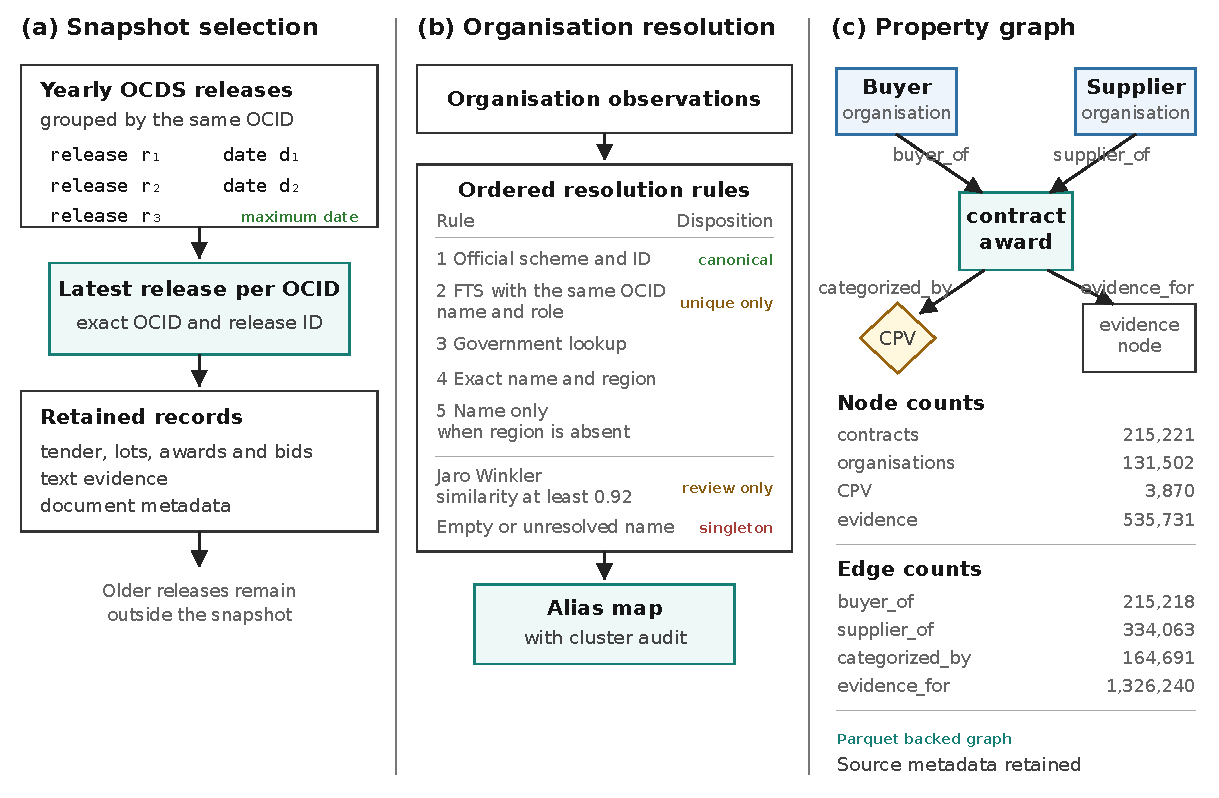
\includegraphics[width=0.88\linewidth]{fig03_data_graph}
  \caption{Construction of the frozen reasoning state.  Snapshot selection precedes rich
  extraction, organisation resolution preserves unresolved singletons and an alias audit, and the
  typed property graph retains record and evidence provenance.  Similarity candidates do not write
  automatic merges.}
  \label{fig:data-state}
\end{figure}

The canonical graph is compiled from typed Parquet tables.  Table~\ref{tab:graph-full} gives the
node and edge counts in the frozen artifact.  All primary key duplicate counts are zero, every
alias target exists, and all edge endpoints resolve to a node.  Historical validation recorded 23
passes, three coverage warnings, and no failures.  The current checkout contains the final graph
tables but not the raw and interim tables needed for a complete rebuild from source releases.

\begin{table}[h]
  \centering
  \caption{Full graph inventory.}
  \label{tab:graph-full}
  \small
  \begin{tabular}{lr@{\qquad}lr}
    \toprule
    Node table & Rows & Edge table & Rows \\
    \midrule
    Contract award & 215,221 & Buyer of & 215,218 \\
    Organisation & 131,502 & Supplier of & 334,063 \\
    CPV & 3,870 & Categorised by & 164,691 \\
    Evidence & 535,731 & Evidence for & 1,326,240 \\
    \bottomrule
  \end{tabular}
\end{table}

The alias map contains 204,711 raw identifiers.  Canonical rows consist of 82,013 singletons,
26,704 deterministic rows, 14,875 name and region merges, 6,332 deterministic safe merge rows,
1,286 name only merges, 255 model adjudicated safe merge rows, and 37 curated government lookup
rows.  The graph contains 76,194 provisional GB FTS singleton identifiers.  GB FTS is not treated
as an authoritative resolved identity even when it remains the key of an unresolved node.

Value extraction stores amount, currency, source, and an additivity flag.  The selected source is a
matching contract for 160,362 rows, an award for 15,640, a tender fallback for 19,623, and missing
for 19,596.  Contract and award sourced rows give 176,002 rows marked additive.  This label means
row additive under the extraction convention and not realised expenditure.  A process with several
matching contract records uses the first deterministic match.  No currency conversion is applied.

Evidence text preserves the source field path and lot identifier.  Exact lot matching is preferred.
When no lot match exists, an OCID level fallback links evidence to awards in the same contracting
process and records that fallback scope.  This supports provenance navigation but not award level
textual entailment.

\section{Recursive Algebra}
\label{app:algebra}

The single call PACS and WTQ protocols use trees over seven return types.  A \records value is a
subset of the record universe, \values is a distinct scalar set, \groups maps keys to numeric
values, and \ranking is an ordered sequence of key and score pairs.  The remaining three types are
numeric, scalar, and Boolean.  Programs have maximum depth 16 and at most 64 nodes.  Every validator
failure identifies both a typed reason and a path into the tree.

\begin{table}[h]
  \centering
  \caption{Closed recursive operator inventory.  The first seventeen nodes define the original
  algebra.  WTQ adds the final row preserving node.}
  \label{tab:operators}
  \small
  \begin{tabularx}{\linewidth}{p{0.16\linewidth}p{0.28\linewidth}X}
    \toprule
    Node & Signature & Semantics \\
    \midrule
    \texttt{filter} & predicates $\rightarrow$ \records & Select records \\
    \texttt{values} & \records $\rightarrow$ \values & Project sorted distinct values \\
    \texttt{count} & \records $\rightarrow$ \numbertype & Count distinct contract identifiers \\
    \texttt{size} & \values $\rightarrow$ \numbertype & Set cardinality \\
    \texttt{sum} & \records $\rightarrow$ \numbertype & Decimal sum under domain guards \\
    \texttt{exists} & \records $\rightarrow$ \booltype & Test non emptiness \\
    \texttt{select} & \records $\rightarrow$ \valuetype & Require one distinct field value \\
    \texttt{extreme} & \records $\rightarrow$ \valuetype & Record argminimum or argmaximum \\
    \texttt{groupby} & \records $\rightarrow$ \groups & Grouped count or sum \\
    \texttt{argext} & \groups $\rightarrow$ \valuetype & Extremal group key \\
    \texttt{top} & \groups $\rightarrow$ \ranking & Top $k$ groups, with $k\leq50$ \\
    \texttt{num} & literal $\rightarrow$ \numbertype & Numeric literal \\
    \texttt{combine} & two numbers $\rightarrow$ scalar & Difference, ratio, addition, or comparison \\
    \texttt{vcompare} & values $\rightarrow$ \booltype & Scalar comparison \\
    \texttt{setop} & two value sets $\rightarrow$ \values & Union, intersection, or difference \\
    \texttt{gcombine} & two group maps $\rightarrow$ \groups & Combine aligned group values \\
    \texttt{keys\_where} & \groups $\rightarrow$ \values & Select keys satisfying a threshold \\
    \texttt{extreme\_rows} & \records $\rightarrow$ \records & Retain all rows tied at an extremum \\
    \bottomrule
  \end{tabularx}
\end{table}

Base predicates are equality, membership, substring containment, existence, and lower or upper
bounds.  Negation applies to one predicate and disjunction combines two or more.  An expression
membership predicate evaluates a child value set and binds it to a field, which makes a derived set
bridge expressible.  Numeric combination supports difference, ratio, and addition; Boolean
comparators support greater, less, greater or equal, less or equal, and equal.

The validator enforces composition, required arguments, and tree size.  Backend field legality,
entity identity, additivity, and currency remain environment contracts checked outside this algebra.
Runtime failures include an unknown field, a non finite or non numeric sum, an empty result, and
multiple values for a requested scalar.  Row preserving extrema keep all ties so that a later scalar
selection fails rather than choosing one arbitrarily.  Counts deduplicate contract identifiers,
group keys exclude null and empty strings, sums accumulate in decimal arithmetic, and ranking ties
use a stable key order.  Answer comparison is type strict, so a Boolean cannot equal numeric one.

\section{Online Runtime Contract}
\label{app:runtime}

The following sequence specifies the evaluated online path.

\begin{enumerate}
  \item Select a schema slice from the question without reading result records.
  \item Produce a typed intent with answer signature, literals, roles, operations, and dependencies.
  \item Validate the intent.  Compile it directly when valid and not vetoed.  Otherwise request a
  conditional typed graph proposal and apply consistency checks.
  \item Ground fields, values, roles, entities, dependencies, exhaustive access, and aggregate
  guards.  Run preflight checks.
  \item Execute variables in dependency order on the frozen record view.  Store intermediate
  population sizes, emitted values, and execution states.
  \item Assemble the answer card and apply evidence, output consistency, postflight, and disclosure
  logic.
  \item If an eligible structured failure occurs and the budget remains, remove oracle and
  reference fields, request one revised proposal, and return to Step 3.  Otherwise release the
  answer or terminate without one.
\end{enumerate}

The current evaluation default is one feedback replan.  Structural resampling inside conditional
planning may draw two proposals after detectable compilation or consistency failure.  The teacher
harvest uses at most two feedback repairs.  Independent variables at the same dependency level may
execute concurrently, but their deterministic denotation and stable reduction order remain fixed.

The main runtime and the recursive algebra are separate implementations.  The runtime exposes
eleven planner facing operation units including abstention, while the single query executor supports
ten direct operations.  Bridge and comparison dependencies use graph or decomposition paths.  PACS
and WTQ instead call the closed recursive evaluator directly.

\section{Prompt, Schema, and Feedback Contract}
\label{app:prompts}

Both learned stages are constructed in
\path{src/procurement_graph/reasoning/typed_planning.py}.  Neither receives database rows or the
answer oracle.  Strict JSON schemas fix the output objects independently of the natural language
instruction.

\paragraph{Structured understanding.}
The Stage 1 system instruction asks for a small typed computation program and explicitly prohibits
answering the question.  Its user payload contains the question, task definition, allowed slots,
operation guidance, hard rules, and a keyword selected schema context.  The answer signature names
the operation, value type, and answer field.  Program steps name their inputs, literal filters,
operation, return kind, and output step.  Unsupported or ambiguous content requires an abstention
with an empty program.

The exact fixed system string is:
\begin{quote}\small
You are the typed intent programmer for a UK public-procurement KGQA system. Convert the question
into a small computation program. Do not answer the question. Use only information explicitly
present in the question. The output shape is enforced by a strict JSON schema.
\end{quote}

Allowed literal slots are publication year or ranges, numeric CPV code, CPV label, the three
procurement categories, buyer, supplier, exact quoted title, explicit dates, and explicit amount
thresholds.  The instruction keeps CPV labels separate from high level procurement categories,
forbids invented literals and invented root inputs, requires later steps to reference preceding
identifiers, and treats future years as executable no result scopes rather than predicted
ambiguity.  Count, existence, and abstention signatures have no answer field.

The schema slice exposes the available node fields, relations, and eleven operation units.  These
are record filtering, distinct projection, count, sum, unique selection, existence, maximum,
minimum, top $k$, comparison, and abstention.  The slice is selected from the question before any
result record is read.

\paragraph{Conditional graph planning.}
Stage 2 receives the question, the Stage 1 briefing, schema context, and capability instructions.
It returns a flat array of typed variables, relations, a return specification, and a reasoning
order.  Variable identifiers encode parent structure when possible.  A conjunction remains one
record variable with several filters.  A bridge must derive an entity set from source records and
bind that set into a target record variable before reduction.  Comparison returns identify left and
right operands, metric, and comparator.  Unused schema fields take empty values and cannot be filled
with invented semantics.

The exact fixed system string is:
\begin{quote}\small
You are the structured graph planner for a UK public-procurement KGQA system. Turn the question and
the Step-1 briefing into an executable graph\_plan (variables + return). A strict schema fixes the
output shape; fill the fields faithfully and never answer the question.
\end{quote}

Two prompt payload variants exist.  The card variant adds an executor capability card and selected
template shell, while the lean variant provides the briefing without that shell.  The variant is a
model configuration choice and must be recorded with a run.  The current historical artifacts do
not preserve one complete arm to prompt manifest, so the paper does not attribute performance to
this choice.

\paragraph{Repair visibility.}
A repair receives the failed proposal and a structured failure object.  The instruction asks for a
revised understanding or plan, prohibits answering, and prohibits inference of hidden references.
All oracle and expected answer values are removed recursively from the payload.  A structural
resample adds a note that the prior graph failed compilation or consistency and requests a different,
simpler decomposition.  This resampling is allowed only for detectable structural defects.  A
program that executes successfully but is semantically wrong cannot be selected for online repair
because the online runtime has no oracle.

The reader repair system string begins, ``You are the repair reading layer for a verifier-guided UK
procurement KGQA system,'' and requires a revised question understanding without an answer or a
hidden reference.  The graph repair string begins, ``You are the repair reflector inside a
verifier-guided KGQA graph planner,'' and requires one allowed repair action followed by an object
under the same graph schema.  The exact emitted strings and dynamic JSON payload are generated by
\texttt{repair\_understanding\_messages} and \texttt{typed\_replan\_messages}; their containing source
hash is reported in Table~\ref{tab:source-hashes}.  For an offline mismatch, the only visible
semantic feedback is that the submitted answer failed external validation.

\section{Failure Taxonomy and Worked Transitions}
\label{app:failures}

Table~\ref{tab:failure-taxonomy} gives mutually exclusive failure families over all 1,725 repair
targets.  The taxonomy assigns each rejection to the first responsible contract rather than
compressing it into wrong answer.  The 242 external validation rows exist only in offline curation.

\begin{table}[h]
  \centering
  \caption{Failure families in the teacher repair corpus.}
  \label{tab:failure-taxonomy}
  \small
  \begin{tabular}{lrl}
    \toprule
    Failure family & Rows & Observation point \\
    \midrule
    Type contract & 907 & Before execution \\
    Offline external validation & 242 & After execution \\
    No confident schema match & 178 & Before execution \\
    Dropped question atom & 136 & Before execution \\
    Multiple answers for scalar & 120 & During execution \\
    Operation contract & 59 & Before execution \\
    Type gate & 38 & Before execution \\
    Invalid graph plan & 18 & Before execution \\
    Execution syntax & 17 & During execution \\
    Empty result & 5 & During execution \\
    Other graph or abstention & 5 & Mixed \\
    \midrule
    Total & 1,725 & \\
    \bottomrule
  \end{tabular}
\end{table}

Four transition patterns clarify the contract.  A correct aggregate proposal carries the buyer or
supplier bridge, preserves all literals, and includes the additive value guard before the executor
sums any records.  A repairable type error may request a monetary answer while returning a record;
grounding rejects it before execution, typed feedback names the incompatible return, and a revised
value extremum is evaluated from the beginning.  An ambiguous scalar request may ground cleanly but
produce several buyers or suppliers; the executor reports multiple answers and the system eventually
withholds an answer rather than choosing one.  Finally, an incomplete bridge can count the source
set, pass every online check, and still disagree with the oracle by orders of magnitude.  The last
case has no online repair trigger and is routed as an offline hard negative.

The stored repair corpus preserves the initial failure, successful target, and round count, but not
every intermediate provider payload.  The following episode therefore distinguishes stored
artifacts from prompt reconstruction and deterministic replay rather than presenting a synthetic
conversation as an original log.

\subsection{A complete teacher failure and offline repair}
\label{app:complete-repair}

Consider benchmark item \texttt{L2::bridge\_join\_0583\#L2a}:
\begin{quote}\small
Just looking at the relevant procurement records, how many contract notices were published by
buyers that went on to award a contract to GLEAM SERVICE CENTRE LTD?
\end{quote}
Its answer is a count.  The benchmark generator executes the latent bridge specification against
the graph snapshot and stores 1,623 as an evaluation oracle.  This value is never included in a
planner or reflector prompt.  The episode is useful because the first proposal is well typed,
grounded, executable, and nonempty, yet it answers a different question.

The complete stored chain is joined by the item identifier across
\texttt{cicada\_core\_v4/train.jsonl}, \texttt{teacher\_full\_v1/traces.jsonl},
\texttt{hard\_negatives.jsonl}, \texttt{repair\_sft.jsonl}, and \texttt{dpo\_pairs.jsonl}.  Their
content hashes appear in Table~\ref{tab:artifact-hashes}.  This identifier based join is preferable
to line numbers, which change when JSONL artifacts are regenerated or sorted.

\paragraph{Initial teacher call and deterministic compilation.}
The first teacher was asked to translate the question into a typed computation program without
answering it.  Its fixed system instruction stated that literals must come only from the question
and that a strict JSON schema controls the output.  The case specific user object contained the
question, the allowed procurement slots, operation guidance, the bridge pattern
\texttt{source records $\rightarrow$ distinct entity set $\rightarrow$ bound target records}, and
the retrieved schema context.  The stored response identified a numeric count, but represented the
request as one filtering step.  In abbreviated form, the artifact reads
\begin{quote}\small\ttfamily
A = filter\_records(\par
\hspace*{1em}supplier is awarded contract to = GLEAM SERVICE CENTRE LTD,\par
\hspace*{1em}buyer publishes contract notice);\par
return A.
\end{quote}
It also marked the meaning of ``contract notice'' as unsupported or ambiguous.  This diagnosis did
not remove the named supplier, but it failed to express that the supplier first determines a set of
buyers and that those buyers then determine the population to count.

This structured response is accepted by the intent program fast path and compiled mechanically.  A
current reconstruction produces a graph exactly equal, field for field, to the historical rejected
graph:
\begin{quote}\small\ttfamily
A = record\_set(supplier = GLEAM SERVICE CENTRE LTD);\par
return count(A).
\end{quote}
The serialized object contains one record variable, no entity variable, and no relation.  Although
its stale template field says \texttt{abstain}, its return operation is \texttt{count}; the runtime
therefore executes the plan rather than treating that label as an answer.  The compact historical
trace does not retain an explicit route tag, but exact reproduction by the deterministic compiler
means that this case does not require, and we do not attribute to it, an initial Stage 2 language
model call.  The configured Stage 2 prompt remains the fallback for intent programs that cannot be
compiled directly.

\paragraph{Initial execution and verdict.}
The executor resolves GLEAM SERVICE CENTRE LTD to a canonical supplier and exhaustively finds 35
matching source records.  The program returns 35.  Grounding, schema checks, operation support,
execution, nonempty evidence, and output shape all pass, so the online verdict is successful.  The
offline teacher run then compares the result with the hidden value 1,623, records
\texttt{oracle\_match=false}, and writes the proposal to the hard negative pool.  Thus the rejection
is not evidence that the online verifier detected a semantic error.  It is direct evidence of the
opposite: executability did not establish constraint faithfulness.

\begin{table}[h]
  \centering
  \caption{Observations in the GLEAM teacher episode.  Historical rows are copied from the stored
  corpus; replay values are recomputed on the versioned graph.}
  \label{tab:gleam-episode}
  \small
  \begin{tabular}{p{0.20\linewidth}p{0.25\linewidth}p{0.43\linewidth}}
    \toprule
    Stage & Observation & Evidence status \\
    \midrule
    Question & Hidden oracle 1,623 & Stored benchmark row \\
    Initial proposal & Count supplier records & Stored teacher trace \\
    Initial execution & 35 records; online checks pass & Stored teacher trace \\
    External audit & 35 does not match 1,623 & Stored teacher trace and hard negative \\
    Repair input & External validation failed; 35 submitted & Reconstructed by the audited repair builder \\
    Repaired execution & $35\rightarrow2\rightarrow1{,}623$ & Stored target plan and current deterministic replay \\
    \bottomrule
  \end{tabular}
\end{table}

\paragraph{Oracle hidden repair.}
The offline curation controller is allowed to use oracle agreement only to decide that another
attempt is warranted.  It then constructs a repair message whose visible semantic content is
equivalent to
\begin{quote}\small\ttfamily
failure\_stage = verifier\par
failure\_reason = wrong\_answer\par
submitted\_answer = 35\par
note = The submitted answer did not match the hidden verifier.\par
note = The reference/oracle answer is intentionally hidden.\par
note = Repair the plan using only the question and trace summary.
\end{quote}
The full object also carries the failed graph, empty grounding and schema failure lists, the online
check summaries, and a closed set of repair actions.  Before prompt construction, keys such as
\texttt{oracle\_answer}, \texttt{gold\_answer}, and \texttt{expected\_answer} are recursively
removed.  The reflector is instructed to diagnose one failure, select one allowed action, preserve
all question literals, and return another graph under the planning schema.  The compact export
stores this signal as \texttt{submitted answer failed external validation}; it does not store the
raw provider completion byte for byte.  The prompt described here is therefore reconstructed from
the committed repair builder and the stored failed trace, while the plans on either side are stored
artifacts.

The accepted repair restores the missing relational path:
\begin{quote}\small\ttfamily
a1 = record\_set(supplier = GLEAM SERVICE CENTRE LTD);\par
b1 = distinct buyer(a1);\par
c1 = record\_set(buyer in b1);\par
return count(c1).
\end{quote}
The executor can now expose every transition.  Variable \texttt{a1} contains the 35 awards to
GLEAM.  Variable \texttt{b1} contains two buyers: London Borough of Haringey, Passenger Transport
Services, and Royal Borough of Greenwich, managed by GS Plus Ltd.  Binding those identities into
\texttt{c1} yields 1,370 and 253 procurement records respectively, hence 1,623 records in total.
For example, the source set contains record
\texttt{contract:ocds-h6vhtk-035eee:022611-2022-1}, titled ``Regular Services'' and carrying CPV
60170000.  The replay trace retains the complete record identifiers and provenance for all three
variables; the paper reports counts rather than printing 1,623 rows.
The final execution again passes the online checks and now also agrees with the hidden oracle.  The
controller consequently exports the repaired plan as supervised data and the repaired and rejected
plans as an oracle curated preference pair.

This episode locates the gain precisely.  The repair does not improve entity grounding or make an
invalid program executable; both properties already held.  It changes the reasoning action by
inserting the omitted supplier to buyer to record bridge.  The environment makes that change and
its consequences inspectable, while the offline oracle supplies only a bounded selection signal.

\section{Benchmark Composition and Integrity}
\label{app:benchmark}

The stored benchmark partitions contain 9,267 training, 671 development select, 556 development
tune, 49 development smoke, and 2,285 final artifact rows.  The total is 12,828.  Every one of the
260 balanced development diagnostic identifiers occurs inside the final artifact.  Removing them
produces the primary 2,025 row set.  This operation is a deterministic identifier exclusion over
the same stored predictions and not a second model run.

The primary set contains 1,725 answerable rows and 100 rows from each non answer class.  The
inclusive artifact contains 1,925 answerable rows and 120 rows from each non answer class.  Whole
plan identifiers do not cross from training to the final partition.  A string audit nevertheless
finds two identical question and answer pairs and five deduplication groups across that boundary,
so the split is plan separated rather than entirely duplicate free.

Stage 1 executes specifications on the production backend and a separate reference index before
surface generation.  Stage 2 checks the naturalised question.  One historical factoid gate sampled
30\% of eligible rows for language model review and marked the unsampled rows verified by default.
The independent evaluator audit concerns answer oracles and does not imply that every natural
language surface received an independent semantic review.

\section{Training Data and Configurations}
\label{app:training}

Table~\ref{tab:training-data} distinguishes harvest counts from final exports.  Repair, preference,
hard negative, and direct target views can overlap.

\begin{table}[h]
  \centering
  \caption{Teacher harvest and training exports.}
  \label{tab:training-data}
  \small
  \begin{tabularx}{\linewidth}{XrX}
    \toprule
    Artifact & Rows & Interpretation \\
    \midrule
    Training questions & 9,267 & One primary trace per question \\
    Answer and online runtime pass & 6,860 & Not an answer correctness label \\
    Oracle agreement before shape & 5,605 & Offline only \\
    Direct graph targets & 5,598 & Oracle and shape accepted pool \\
    Hard negatives & 1,262 & 1,021 oracle and 241 shape mismatch \\
    Repair targets & 1,725 & Overlapping successful repair view \\
    Preference pairs & 390 & Accepted and rejected candidates \\
    Abstention targets & 590 & Correct non answer pool \\
    Plan SFT export & 2,787 train, 57 validation & Includes capped abstentions \\
    Repair SFT export & 1,679 train, 46 validation & Successful repairs \\
    Step 1 export & 5,091 train, 96 validation & Structured intents \\
    \bottomrule
  \end{tabularx}
\end{table}

Every main adapter uses 4 bit QLoRA with rank 64, alpha 128, dropout 0.05, bfloat16 compute, all
target modules, cosine decay, and effective batch size 16 \citep{hu2022lora,dettmers2023qlora}.
The initial plan and repair SFT stage trains for three epochs at learning rate $10^{-4}$ with a
6,144 token cutoff.  Qwen rejection sampling continuation uses 3,019 plan and 3,169 repair rows;
Llama uses 3,026 and 3,190.  Both train for two epochs at $5\times10^{-5}$.  Qwen DPO uses 1,079
pairs and Llama 1,083, each for one epoch at $5\times10^{-6}$ with $\beta=0.1$.  Serving logs record
vLLM 0.24.0, seed 0, bfloat16, maximum length 8,192, and disabled Qwen thinking
\citep{kwon2023vllm}.  A formal GPU model manifest is not preserved.

The historical teacher summary stores the Step 1 and Step 2 model names but not a full command,
prompt hash, worker count, or complete call parameters.  Temperature zero and the reported budgets
are reconstructed from the audited runner.  Teacher resume is not transactional because a trace may
be written before all downstream supervision views.  The preserved corpus counts above are the
audited artifact facts.

\section{PACS and WikiTableQuestions Protocols}
\label{app:external-protocols}

The external evaluations deliberately reuse the recursive action language but not the full
procurement runtime.  In particular, neither protocol invokes the two stage procurement planner,
the entity grounder, the procurement evidence retriever, or the online repair loop.  Each question
is presented once to a model that emits one recursive tree.  The tree is parsed, type checked, and
executed by the deterministic evaluator.  This separation is necessary for interpreting the
results as tests of the representation and its supervision rather than as replications of the
complete environment.

\paragraph{PACS construction.}
PACS is an intent balanced procurement challenge set.  Its seven families cover spending and
volume, temporal change, supplier concentration, cross buyer comparison, overlap and exclusion,
relational composition, and disclosure or compliance.  Complexity is recorded independently as
atomic, simple, or nested.  Each intent is rendered as paired surfaces while retaining the same
gold tree and oracle.  Surface A uses an independently authored canonical grammar.  Surface B is a
naturalised rendering subjected to literal and logic preservation checks.  The third training
renderer is diagnostic and is not reported as a primary surface.

The corrected v1.1 evaluation contains 922 intent instances.  Of these, 730 are answerable, 138
request unsupported or ambiguous content, and 54 have an executable no result scope.  These labels
replace an earlier transformation that classified 36 false or zero valued answerable denotations as
no result.  The correction joins stored trees by identifier and replays them on the frozen backend;
it does not regenerate model outputs.  The current repository does not contain the correction script
or corrected item level correctness fields, so only the corrected aggregate counts are treated as
authoritative.

The intended decoding contract is one call, temperature zero, at most 1,200 generated tokens, and
no reflection.  The current runner defaults to prompt only JSON and offers guided decoding only as
an explicit flag.  The historical result bundle does not retain its complete launch command,
however, so the paper does not use guided versus unguided decoding as an explanatory variable.  The
seal also lacks a separate template identity gate and its trigram screen samples every seventh
training trigram set.  PACS is consequently described as a frozen compositional diagnostic, not as
a fully sealed structural out of distribution test.

\paragraph{WTQ conversion and scoring.}
For WikiTableQuestions, every table is converted into a typed record view.  Column names form the
schema, cell strings remain available to the model as hints, and execution is restricted to the
table associated with the question.  The pristine unseen table split contains 4,344 questions over
421 tables not observed in the corresponding training views.  The model receives cell hints and
emits one tree with no reflection.  Compared with the procurement algebra, the table executor adds
\texttt{extreme\_rows} so that all rows tied at a maximum or minimum can flow into later operators.

Official evaluation is performed only after serialisation.  Tabs and newlines inside an answer item
are replaced with spaces, answer items are joined with tabs after the question identifier, and the
result is passed to the WikiTableQuestions evaluator v1.0.2 with the CoreNLP tagged targets.  The
internal JSON \texttt{correct} field is not used for Table~\ref{tab:external}.  The frozen run used
Qwen3 8B with thinking disabled, bfloat16 inference, maximum model length 8,192, LoRA rank 64,
concurrency eight, cell hints, and no reflection.  The source manifest records commit
\nolinkurl{17993565347e78be3507657bfef941264050d7aa}.  The official target directory and the exact final
translated program training snapshot are absent from this checkout, preventing a clean current
machine reproduction of the official scores.

\paragraph{Metric semantics.}
For both protocols, a parsed program is insufficient for correctness.  The program must type check,
execute, return the expected answer kind, and agree with the oracle under the protocol specific
normaliser.  PACS reports strict corrected item accuracy.  WTQ reports the official evaluator's
denotation accuracy.  Paired McNemar tests compare item correctness vectors for two checkpoints;
they do not measure variation across training seeds.

\section{Additional Results and Statistical Scope}
\label{app:results}

For continuity, the inclusive 2,285 row scores are 16.63\% for closed book, 25.56\% for plan guided
RAG, 39.21\% for top 40 RAG, 69.76\% for the cloud teacher, 75.97\% for hybrid Llama, 78.03\% for
hybrid Qwen, 83.33\% for fully local Llama, and 85.65\% for fully local Qwen.  These predictions
contain the 260 development questions and are not the primary confirmatory comparison.

The balanced 260 row diagnostic gives 155 correct for the deterministic KG only planner, 82 for
naive RAG, 75 for strong RAG, 192 for the stored third teacher replicate, 224 for fully local Qwen,
and 219 for fully local Llama.  Fully local Qwen changes 73 KG only errors to correct and four
successes to wrong, with exact McNemar $p=1.89\times10^{-17}$.  Bridge questions change from 7 of
20 under KG only rules to 14 of 20, and top $k$ questions from 1 of 20 to 18 of 20.  These are
development diagnostics.

A separate WTQ development diagnostic samples four candidates for each of 300 questions after basic
program checks.  The first temperature zero candidate scores 59.00\%.  Selecting the first verified
candidate scores 57.33\%, a deterministic scorer using six execution derived fault features scores
59.33\%, and an oracle selector reaches 62.33\%.  A faithful language model judge with access to the
executed answers produces no gain over its own first candidate baseline, while an immediate language
model score is 0.66 points worse.  This result motivates deterministic diagnosis but is not part of
the single call WTQ result in Table~\ref{tab:external}.  It changes both the sampling budget and the
selection procedure, and its historical aggregates are not bound to the pristine test manifest.

The grounding audit begins with 136 saved proposals that have typed oracles.  Its fourteen rescues
all insert the additive sum guard.  The constraint audit begins with 237 repairs associated with
schema, runtime specification, or entity grounding.  It can mechanically map question constraints
for 229.  Among the 56 flagged targets, category is absent in 43, buyer in six, supplier in three,
signed date in three, title in two, and CPV in two.  Categories can overlap within one target.

PACS corrected v1.1 contains 922 rows.  The earlier stored summaries report 332, 450, 687, and 675
correct for base A, teacher A, Compose A, and Compose B.  The corrected aggregate reports 312, 470,
722, and 711.  Only the corrected values are used in the paper.  The transformation concerns 46
rows over development and test, including 36 test rows.  The saved prediction files retain the old
per item correctness field, which is why the corrected aggregates cannot be independently rebuilt
from those fields alone.

WTQ official scoring uses 4,344 saved answer item rows for each arm.  The official paired counts are
387 gains and 178 losses from base to procurement Compose, 833 and 90 from Compose to answer matched
training, and 628 and 308 from answer matched to translated gold training.  The answer matched
training snapshot has 4,615 train and 94 validation rows.  The translated gold snapshot contained
about 5,423 rows, but the exact final version is missing.

\section{Running Example Provenance}
\label{app:running-example}

Figure~\ref{fig:motivation} asks how many contract notices were published by buyers that had awarded
a contract to Edmundson Electrical Limited.  Its deterministic denotation can be reconstructed from
the frozen record view without a model.  Filtering \texttt{supplier\_name} by the exact supplier
string returns 23 distinct contract notices.  Projecting and deduplicating their buyer names returns
16 buyers.  Filtering the same frozen view by those buyer names returns 4,257 distinct contract
notices.  These three counts have been independently rerun against the graph hashes in
Table~\ref{tab:artifact-hashes}.

The retrieval reader answer of 14 and the untrained one shot answer of 23 are historical model
outputs represented in the figure.  Their complete raw responses, retrieved row identifiers, model
revision, and launch command are not preserved as one trace bundle in the current checkout.  The
existing \path{scripts/paper_figures/fig1_trace.py} targets a different PACS bridge question and
therefore cannot be used as provenance for these two panels.  The figure supports the conceptual
distinction between a finite observation, a valid one hop action, and the complete two hop
denotation.  It is not included in the quantitative system comparison and the two historical model
outputs should be regenerated and archived before an artifact release.

\section{Reproduction Protocol}
\label{app:reproduction}

This section distinguishes three increasingly strong reproduction targets.  A graph validation
reproduction starts from the eight frozen Parquet files and reruns all structural checks.  A saved
prediction reproduction recomputes metrics and paired statistics without calling a model.  A full
experimental reproduction additionally requires the original inputs, checkpoint adapters, launch
arguments, and external target resources.  Only the first two targets are complete for the primary
paper claims in the current checkout.

\subsection{Software environment}

The core package requires Python 3 with pandas at least 2, pyarrow at least 14, PyYAML at least 6,
jellyfish at least 1, tqdm at least 4, the OpenAI client at least 1, azure-identity at least 1.16,
pytest at least 8, FastAPI at least 0.110, and uvicorn at least 0.29.  Training additionally used
LLaMA-Factory with its PyTorch and metrics extras.  Serving logs identify Transformers 5.6.0 and
vLLM 0.24.0.  These versions are historical observations rather than a complete lock file.  API
credentials are read from environment variables and are never written to traces.

The audit reference is commit \nolinkurl{d15ec0a3bd5b5f295f9828e44067094b73ab2cd7}.  Because the
audited worktree contained staged data and later correctness fixes, the commit alone is not a release
identifier.  Tables~\ref{tab:artifact-hashes} and~\ref{tab:source-hashes} therefore bind the paper to
content hashes in addition to a commit.

\subsection{Data build and validation}

A complete source build proceeds in the following order.  Ingestion chooses the latest release for
each process and normalises the five annual OCDS files.  Entity resolution then creates deterministic
components, emits conservative similarity candidates, and applies only reviewed safe decisions.
Rich extraction creates contract, organisation, CPV, value, and evidence tables.  The graph builder
materialises typed nodes and edges, after which the validator checks primary keys, endpoints,
cardinality, and coverage.  The commands are:

\begin{verbatim}
python -B pipelines/01_ingest.py
python -B pipelines/02_er_phase1.py
python -B pipelines/03_er_phase2.py
python -B pipelines/04_extract.py
python -B scripts/apply_safe_er_merges.py
python -B pipelines/40_build_kg.py
python -B pipelines/41_validate_kg.py
\end{verbatim}

These commands specify control flow but are not currently sufficient for a source rebuild because
the raw annual releases, intermediate extraction tables, and reviewed merge decision files are not
present.  Starting from the frozen graph files is reproducible.  A successful validation must obtain
the row counts in Table~\ref{tab:graph-full}, zero duplicate primary keys, no missing alias target,
and no unresolved edge endpoint.  Coverage warnings are reported but do not mutate the graph.

\begin{table}[h]
  \centering
  \caption{SHA256 hashes of the frozen reasoning state.}
  \label{tab:artifact-hashes}
  \scriptsize
  \begin{tabularx}{\linewidth}{p{0.29\linewidth}X}
    \toprule
    File & SHA256 \\
    \midrule
    \texttt{contract\_nodes.parquet} & \nolinkurl{246caad93e1c8b184d3714a280190efb3c238f4cab73cd3bf1f36b38de307bf1} \\
    \texttt{org\_nodes.parquet} & \nolinkurl{42f9542833275ea7a57feb2cc4f4e64a507513f35b2e420a449d938b68b867af} \\
    \texttt{cpv\_nodes.parquet} & \nolinkurl{5cfc3ce5c201b4d683a68ac92b192a469541768f82a153b2d93ef11a6e276336} \\
    \texttt{evidence\_nodes.parquet} & \nolinkurl{45c9a5f9c50b8859f5d932e4f6ece59ec6cfe97741728b56c7807c9e46f1afbe} \\
    \texttt{buyer\_of.parquet} & \nolinkurl{43133080caf07e393b1e277fdfe970cedbd599ec7209b2b4f3229988be3e492a} \\
    \texttt{supplier\_of.parquet} & \nolinkurl{857617e0fd09919ba09146905f1ceccb0e84d6d42a34522c7ca2d015102f0fb8} \\
    \texttt{categorized\_by.parquet} & \nolinkurl{bc13646e8a45117e085f41b9479baba0e7d21f15526f7e6b4527df2f96859e0d} \\
    \texttt{evidence\_for.parquet} & \nolinkurl{1a66a5ce3722d932506df2b429514f48adcd5811146e5107d922860d73ca1640} \\
    \bottomrule
  \end{tabularx}
\end{table}

\subsection{Teacher collection and supervision export}

The teacher input is \path{data/qa/cicada_core_v4/train.jsonl}, containing 9,267 rows with SHA256
\nolinkurl{3a9906a934c092a629d3f1d502a3e146dd15093a74173ab52897ae1c16a7f5a1}.  The preserved
\path{data/qa/teacher_full_v1/traces.jsonl} has SHA256
\nolinkurl{cbbd6e2e3fe45a4c4c4fc1d94ff115e4d655905b12bc3088db591e1c486cd1bb}.  A representative
invocation reconstructed from the audited runner is:

\begin{verbatim}
python -B scripts/run_teacher.py \
  --questions data/qa/cicada_core_v4/train.jsonl \
  --out-dir data/qa/teacher_full_v1 \
  --step1-model gpt-5.4-nano \
  --plan-model grok-4-1-fast-non-reasoning \
  --plan-temperature 0 --plan-samples 2 \
  --max-repairs 2 --resume
\end{verbatim}

The Step 1 temperature is also zero in the client.  The Grok model name selects the lean prompt and
optional schema profile.  Each API call has a 60 second timeout and at most three retries after the
first attempt, waiting two, four, and six seconds.  No explicit generation token cap is passed, so
the provider default applies.  The original worker count is not recoverable: a worklog describes an
eight worker resumed run while the current command default is four.  Concurrency changes completion
order and rate limit exposure but should not change a successful temperature zero response; it must
nevertheless be logged in a new release.

Strict provider JSON schemas constrain Step 1, Step 2, and repair outputs.  Recoverable schema errors
may fall back to JSON extraction and are marked in the trace.  Two structural plan samples are not a
best of two oracle selection.  A second sample is requested only after a detectable compilation or
consistency error.  Offline answer disagreement can initiate a repair, but the repair sees only the
statement that external validation failed.  Hidden answer fields are recursively removed.

After harvest, \path{scripts/export_llamafactory.py} constructs direct, repair, rejection sampled,
and preference views using family and bucket caps.  \path{scripts/export_step1_sft.py} constructs the
intent view.  The stored export counts in Table~\ref{tab:training-data} are required invariants.
Views overlap by design, so their row counts must not be added to estimate the number of unique
questions.  Exported metadata containing the label \texttt{executor\_verifier} is stale for direct
SFT rows; the actual branch also requires offline oracle and answer shape agreement.

\subsection{Training and serving}

Training is launched with \texttt{llamafactory-cli train} followed by one of the seven configuration
files in Table~\ref{tab:config-hashes}.  Relative model, dataset, output, and logging paths inside a
configuration must be resolved from the repository root.  A new run should additionally record the
base model revision, tokenizer revision, CUDA and driver versions, GPU type, random seed, final
adapter hash, and the exact selected checkpoint.  The historical logs establish one CUDA process
and the schedules in Appendix~\ref{app:training}, but do not establish the GPU model.

\begin{table}[h]
  \centering
  \caption{Audited training configuration hashes.}
  \label{tab:config-hashes}
  \scriptsize
  \begin{tabularx}{\linewidth}{p{0.34\linewidth}X}
    \toprule
    Configuration & SHA256 \\
    \midrule
    \texttt{qwen3\_8b\_sft\_qlora.yaml} & \nolinkurl{832802774952da5c691dc8c154627f8f60d10fc0c844dccf500a405a9df2a1bc} \\
    \texttt{llama31\_8b\_sft\_qlora.yaml} & \nolinkurl{6bbf69e6c5d2782764255e0c3fc8c6320bd47af504d97a56f529fad79f2d1171} \\
    \texttt{qwen3\_8b\_rsft\_qlora.yaml} & \nolinkurl{a2c564579828d4056bb3637e7dbbd8cc2c5878f52aea53d45c0d4f56f29d9f09} \\
    \texttt{llama31\_8b\_rsft\_qlora.yaml} & \nolinkurl{4c95235ecf845f2e24406d342b61e7d995b740aa20ef41b8541496e444068a65} \\
    \texttt{qwen3\_8b\_dpo\_qlora.yaml} & \nolinkurl{5b7a115491b98f03d3a7245b7956ec810ffbc9392c90e0658aae8601ac715dbe} \\
    \texttt{llama31\_8b\_dpo\_qlora.yaml} & \nolinkurl{2119cde4f58fd5738913d30e841cc8c8f2e0319b53d5292c3c37afa312da0cef} \\
    \texttt{qwen3\_8b\_compose\_sft\_v3\_qlora.yaml} & \nolinkurl{1d7ada7597ac8395a252e8a6872ed6c8c5e68098caa06c3bc61827367646ec08} \\
    \bottomrule
  \end{tabularx}
\end{table}

The evaluation server uses bfloat16, maximum context length 8,192, LoRA rank 64, and seed zero.
Qwen thinking is disabled through the chat template.  The procurement comparison runner is
\path{scripts/run_compare.py}.  Every arm must record the input file, system mode, planner mode,
Step 1 model and adapter, Step 2 model and adapter, base URL, retrieval mode and $k$, repair flag,
worker count, and output directory.  The historical eight arm result directories do not preserve a
complete mapping of these values, which is why the primary table is labelled a stored system
comparison and not an exactly reconstructed current HEAD run.

\subsection{Metric reconstruction and tests}

The primary procurement result is obtained without model calls.  Join every stored prediction to
the benchmark by stable identifier, remove the 260 development identifiers, and apply the same
typed answer normaliser to all arms.  The resulting set must contain 2,025 rows with the class counts
reported in Appendix~\ref{app:benchmark}.  Accuracy is the mean item correctness.  Answerable and
non answerable rows use different contracts: denotation agreement for the former and exact status
agreement for the latter.  Pairwise significance uses the two discordant cells of the item level
correctness table and a two sided exact McNemar test.  No independence assumption is made across
surface renderings or derived status variants.

The 260 row checkpoint ladder is development evidence.  The same identifiers, runtime, repair
budget, and scorer are used at each rung, but each checkpoint represents one training run.  PACS
correction replays the already emitted trees.  WTQ requires the exact answer item serialisation and
official scorer described in Appendix~\ref{app:external-protocols}.  Running
\texttt{python -B -m pytest -q} on the audited current implementation passes 483 of 483 tests; this
checks code contracts and does not reproduce any learned model result.

\begin{table}[h]
  \centering
  \caption{Audited implementation source hashes.}
  \label{tab:source-hashes}
  \scriptsize
  \begin{tabularx}{\linewidth}{p{0.30\linewidth}X}
    \toprule
    Source & SHA256 \\
    \midrule
    \texttt{typed\_planning.py} & \nolinkurl{adb9c5ef58dfc3efa775f751c80f98f5885181be0f0ad51db323fbfb33a82980} \\
    \texttt{chat.py} & \nolinkurl{001f0c5415c6b0dee237dbb3b210f41b52f20a2a4078f43632f3b05454eee81c} \\
    \texttt{run\_teacher.py} & \nolinkurl{ae0278f23b130ebe4065b6e717acf8ba4209e37bf53b8875ebd3e1731c3a4b23} \\
    \texttt{export\_llamafactory.py} & \nolinkurl{d5c946d788f2f72e556c04abc605e7a402178bd583fa4bfe688303a45d8942a1} \\
    \texttt{export\_step1\_sft.py} & \nolinkurl{fb30c2429ec8d1ff810c2905537c012f4e3a23285c88df83ea3ebfca10190e24} \\
    \texttt{run\_compare.py} & \nolinkurl{5a3c90e74c8e8232e0f40cbc1bbf99b3a32b78bafb9db00b723012f9299b834c} \\
    \texttt{eval\_ladder.sh} & \nolinkurl{a49a05fc69bca068c9006161a48065afd541b089e965c8d31c72b582a66dbc42} \\
    \bottomrule
  \end{tabularx}
\end{table}

\subsection{Minimum release manifest}

For every future arm, the release manifest should contain one immutable record with the source
commit and dirty diff, input and output hashes, base and adapter revisions, prompt builder and schema
hashes, complete command line, environment lock, hardware, seeds, decoding controls, retry policy,
start and end time, interrupted and resumed identifiers, scorer hash, and the derived table cells.
Each answer row should retain the question identifier, snapshot identifier, raw model text, parsed
program, validation events, grounding changes, intermediate population sizes, final denotation,
provenance identifiers, release verdict, and offline labels in separate fields.  This is the minimum
record required to replay an action and attribute a changed outcome without giving the online agent
access to the answer oracle.

\section{Artifact and Reproduction Boundary}
\label{app:artifacts}

The principal implementation entry points are \path{pipelines/01_ingest.py} through
\path{pipelines/04_extract.py}, followed by \path{pipelines/40_build_kg.py} and
\path{pipelines/41_validate_kg.py}.  Safe reviewed entity merges are applied by
\path{scripts/apply_safe_er_merges.py}.  The full runtime uses \path{scripts/run_compare.py}; teacher
curation uses \path{scripts/run_teacher.py}; recursive algebra evaluation uses
\path{scripts/run_compose_probe_eval.py}; and fixed plan grounding analysis uses
\path{scripts/analyze_grounding_impact.py}.

The current repository preserves the final graph, teacher harvest, grounding audits, PACS raw
predictions, and WTQ saved predictions.  It does not preserve the procurement eight arm output
directories, raw and interim graph inputs, reviewed entity merge decision files, corrected PACS per
item artifact, official WTQ target directory, or the exact final translated WTQ training snapshot.
Accordingly, the paper distinguishes direct current artifact audits, deterministic saved prediction
rescoring, and aggregate historical results.

A release suitable for independent reproduction should bind the source commit, data hashes,
checkpoint hashes, prompts, decoding settings, scorer version, and artifact lineage in one manifest.
Teacher collection should write traces and supervision views transactionally.  A matched feedback
attribution experiment should additionally preserve the same initial proposal across no repair,
generic reflection, structured runtime feedback, and offline validation conditions.

\begin{table}[h]
  \centering
  \caption{Evidence and wording boundaries.}
  \label{tab:evidence}
  \small
  \begin{tabularx}{\linewidth}{p{0.23\linewidth}p{0.20\linewidth}p{0.17\linewidth}X}
    \toprule
    Evidence & Control & Runs & Supported wording \\
    \midrule
    Procurement primary & Same 2,025 questions and scorer & One saved pass per arm & Best among
    the stored complete systems \\
    Fixed plan grounding & Question, plan, graph, executor fixed & Deterministic replay & Direct
    effect of one additive sum guard \\
    Checkpoint ladder & Same 260 questions and runtime & One training run per checkpoint & Observed
    cross base SFT improvement and non monotonic later stages \\
    PACS & Frozen one shot diagnostic and saved tree replay & One pass per arm & Compositional and
    surface robustness under the qualified protocol \\
    WTQ & Official test scorer and stored predictions & One pass per checkpoint & Portability of
    the recursive algebra under a table adapter \\
    \bottomrule
  \end{tabularx}
\end{table}

\end{document}
